% !TEX root = ../notes_template.tex

\chapter{복소수와 기하학적 의미}


이 장에서는 복소해석학을 펼칠 무대를 만들기 위해
다음 3가지 중심 주제를 다룬다.

\begin{itemize}
\item[(1)] 복소수의 집합과 연산을 정의하고 실수체의 확장으로서 복소수체 $\mathbb C$를 만든다.
\item[(2)] $\mathbb C$의 원소는 평면 $\mathbb R^2$위의 점으로 표시할 수 있으며, 복소수체 $\mathbb C$의 연산에 대하여
기하학적 의미를 부여할 수 있다. 복소수체와 평면위의 점의 대응 관계로부터
$\mathbb C$에 평면의 유클리드 위상을 가져올 수 있다.
\item[(3)] 끝으로 복소해석학의 기초함수인 지수함수를 공부한다.
또한, 지수함수와 관련된 기본함수인 삼각함수와 로그함수도 살펴본다. 
\end{itemize}

\section{복소수체}

{\bf 복소수}는 실수의 순서쌍으로 정의한다. 예를 들면,
$$
(1,0), \ (0,1), \ (0,0), \ \left(-\dfrac34, \sqrt{2} \right)
$$
는 모두 복소수로 간주할 수 있다.
복소수 전체의 집합 $\mathbb R \times \mathbb R$을 $\mathbb C$라 표기한다. 즉,
$$
\mathbb C = \left\{ z = (x,y) \,:\, x\in \mathbb R, \text{ 이고 } y\in \mathbb R \right\}.
$$

복소수 $z=(x,y)\in \mathbb C$ ($x,y \in \mathbb R$)에 대하여
실수 $x$는 $z$의 실수부, $y$는 $z$의 허수부라고 한다.

집합 $\mathbb C$의
복소수 $(x_1, y_1)$, $(x_2, y_2)$에 대하여
덧셈 ``$+$''과 곱셈 ``$\cdot$''을 다음과 같이 정의한다.
\begin{gather*}
(x_1, y_1) + (x_2, y_2) = (x_1+x_2, y_1+y_2), \\
(x_1, y_1) \cdot (x_2, y_2) = (x_1x_2 - y_1y_2, x_1y_2 + x_2y_1).
\end{gather*}
이 연산에 따라 $\mathbb C$는 체(field)가 된다. 즉,
\begin{itemize}
\item[(F1)]  $(\mathbb C, +)$는 가환군(Abelian group)이다.
\item[(F2)] $(\mathbb C\setminus \{0\}, \cdot)$는 가환군이다.
\item[(F3)] $a,b,c\in\mathbb C$에 대하여 분배법칙이 성립한다:  $(a+b)\cdot c = a\cdot c + b\cdot c$.
\end{itemize}

(F1)에서 가환군이란
연산 $+$에 대하여 결합법칙, 교환법칙이 성립하며,
모든 $(x,y)$에 대하여
$$
(x,y) + (0,0) = (x,y) = (0,0) + (x,y)
$$
를 만족하는 
항등원 $(0,0)$과 
$$
(x,y) + (-x,-y) = (0,0) = (-x,-y) + (x,y)
$$
를 만족하는 덧셈의 역원 $(-x, -y)$이  존재한다는 뜻이다.

유사하게, (F2)에서 곱셈의 항등원 $(1,0)$이 존재하고, 복소수 $(x,y) \in \mathbb C \setminus\{0,0\}$의
곱셈의 역원은 다음과 같다.
\begin{equation} \label{eq:1.1}
\left( \dfrac{x}{x^2+y^2}, \dfrac{-y}{x^2+y^2} \right).
\end{equation}

\begin{salt_exercise}
식 \eqref{eq:1.1}\이 복소수 $(x,y) \in \mathbb C \setminus\{0,0\}$의 곱셈의 역원이 됨을 직접 확인하라.
\end{salt_exercise}


\begin{salt_prop}
$(\mathbb C, +, \cdot)$는 체(field)이다.
\end{salt_prop}

실수  $\mathbb R$은 복소수 $\mathbb C$에 ``포함된다''.
실제로, 복소수 $\mathbb C$안에 $\mathbb R$을 넣어
실수 $\mathbb R$을 $\mathbb C$의 부분체(subfield)로 볼 수 있다.
$$
x \mapsto (x,0)
$$
을 이용하여 실수 $x$를 복소수 $(x,0)$로 보내는 대응 규칙은
단사인 체의 준동형사상(field homomorphism)이다.
즉, 덧셈과 곱셈이 보존되며 서로 다른 실수는 다른 복소수에 대응시키는 사상이다.

\begin{center}
\begin{tabular}{|ccc|} \hline
$\mathbb R$ & & $\mathbb C$ \\ \hline \hline
$x$ & $\mapsto$ & $(x,0)$ \\ 
$x_1+x_2$ & $\mapsto$ & $(x_1+x_2,0) = (x_1,0) + (x_2,0)$ \\ 
$x_1\cdot x_2$ & $\mapsto$ & $(x_1\cdot x_2,0) = (x_1,0) \cdot (x_2,0)$ \\ 
$1$ & $\mapsto$ & $(1,0)$ \\
$0$ & $\mapsto$ & $(0,0)$ \\
\hline
\end{tabular}
\end{center}

따라서 이 사상을 이용한 동일화에 따라 모든 실수는 복소수로 볼 수 있다.
예를 들어 실수 $\sqrt{2}$는 복소수 $(\sqrt{2},0)$로 볼 수 있다.
이런 생각에 익숙하지 않을 수도 있겠으나 우리는 이미 초등학교 과정에서
비슷한 동일화를 경험한 적이 있다. 정수를 유리수의 일부로 동질화하는
다음 예를 보자.
$$
\mathbb Z  \ni 3 = \frac31 \in \mathbb Q
$$
이를 이해하려고 밤잠을 설친 적은 없지 않은가!

실수 해 $x\in\mathbb R$를 갖지 않는 방정식
$$
x^2+1=0
$$
을 복소수 밤위에서 다루면 해를 구할 수 있다.
$$
(0,1)\cdot (0,1) + (1,0) = (-1,0) + (1,0) = (0,0).
$$
$(0,1)$을 나타내는 특별한 기호로 $i$를 도입하면 이 방정식을 다음과 같이 쓸 수 있다.
$$
i^2+1=0,
$$
여기서 실수 $1$과 $0$은 각각 복소수 $(1,0)$과 $(0,0)$에 대응된다.

이제부터 실수  $x,y$로 만든 복소수 $(x,y)$를 $x+yi$로 쓰자.
$$
(x,y) = \underbrace{(x,0)}_{\equiv x} +  \underbrace{(y,0)}_{\equiv y}
\cdot  \underbrace{(0,1)}_{\equiv i} = x+yi.
$$
복소수 곱셈은 교환법식이 성립하고, 특히 $yi = iy$이므로,
$x+yi = x+iy$이다.

\begin{salt_exercise} %1.2
$\theta \in \left(-\dfrac{\pi}2, \dfrac\pi2 \right)$에 대하여
$\dfrac{1+i\tan\theta}{1-i\tan\theta}$를 $x+yi$ 꼴로 표시하면?
\end{salt_exercise}

{\bf 복소수 발견의 역사: }
대중적인 믿음과는 달리 역사적으로 수학자들이 복소수를 진지하게 받아들이게 된 것은 
2차 방정식이 아니라 3차 방정식을 풀 필요가 있었기 때문이다. 요지는 다음과 같다.
16세기 경 포물선 $y=x^2$과 직선 $y=-bx-c$의 교점을 구하는  방법으로 
 방정식
$$
ax^2 + bx + c = 0
$$
을 풀려는 시도가 있었다. 
이러한 기하학적 해석에 근거하여,
포물선  $y=x^2$ 이 직선 $y=-1$과 만나지 않으므로
$x^2+1=0$와 같은 실계수 2차방정식의 해결가능성을 포기하는 것은 쉬운 일이었다.
%%%%%%
그림 \ref{fig-1-1}의 왼쪽 그래프를 참고하라.

\begin{figure}[!h]
\begin{center}
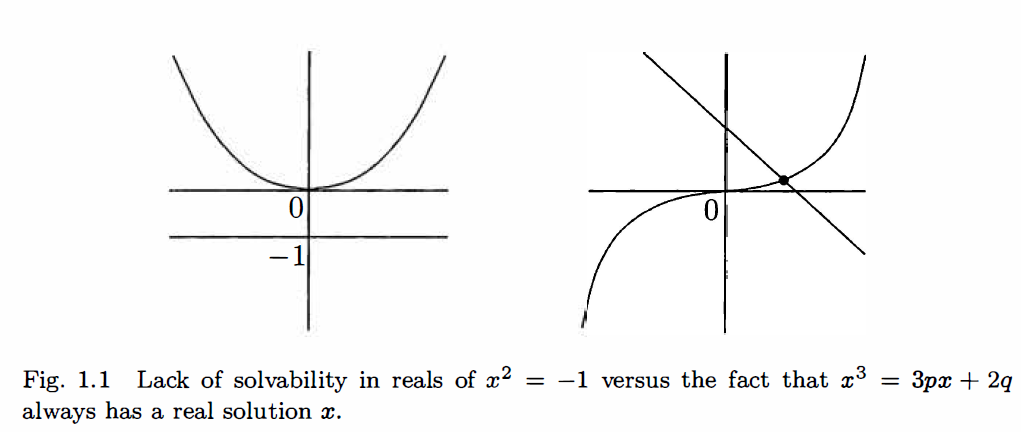
\includegraphics[width=0.6\textwidth]{./SaltChapter/preface-fig-1-1}
\end{center}
\caption{복소함수 $F$와 $G$의 특이점}
\label{fig-1-1}
\end{figure}





